% 11b_capacity.tex: capacity reasoning, follows the strength sections of chapter 11
\section{Capacity and failure order}\label{sec:capacity}\label{sec:strength-capacity}

Capacity design (\cref{sec:loads-capacity}) asks that the arm fail before the joint and the centre body, with a margin of 1.5 on the failure force. The check is geometric: it compares the strength of each arm section with the strength of the joint, both for the same load, a vertical force at the arm tip.

\subsection{Failure force of an arm section}

A vertical force $F$ at the motor axis, at a distance $u_m = \SI{74.25}{mm}$ from the frame centre along the arm, bends every section of the arm at a position $u$ with a lever $u_m - u$:
\begin{equation}
M(u) = F\,(u_m - u).
\end{equation}
A section of elastic section modulus $Z = I/c_\text{max}$ (second moment of area about its horizontal centroidal axis, divided by the largest vertical distance from that axis) reaches the in-plane strength when $M = S_{xy} Z$. The tip force that fails the section at $u$ is therefore
\begin{equation}
F_\text{arm}(u) = \frac{S_{xy}\, Z(u)}{u_m - u}.
\end{equation}
The arm fails at the section where $Z/(u_m - u)$ is smallest, which is not necessarily where $Z$ is smallest: a slim section close to the tip has a short lever.

\subsection{Failure force of the joint}

The joint carries a vertical moment of $M_j = \SI{21216}{N.mm}$ by bearing at its two bolts (\cref{sec:arch-joint}). Its own lever to the motor axis is $u_m - u_j$, with the bolt line at $u_j = \SI{37.24}{mm}$, so the tip force that fails it is
\begin{equation}
F_\text{joint} = \frac{M_j}{u_m - u_j} = \frac{21216}{37.00} = \SI{573}{N}.
\end{equation}

\subsection{Why the planning rule was not conservative}

At the planning stage the requirement was written as a limit on the section modulus at the fork exit, $Z \leq M_j/(1.5\,S_{xy}) = \SI{260}{mm^3}$. That rule compares moments at the same section, as if arm and joint had the same lever. They do not: the fork exit is outboard of the bolt line, so for the same tip force it carries a smaller moment. Requiring the arm's failure force at the fork exit ($u = \SI{43.74}{mm}$) to be at most $F_\text{joint}/1.5$ gives
\begin{equation}
\frac{S_{xy}\, Z}{u_m - u} \leq \frac{1}{1.5}\,\frac{M_j}{u_m - u_j} \quad\Rightarrow\quad Z \leq 260\,\frac{u_m - u}{u_m - u_j} = 260 \times \frac{30.51}{37.01} = \SI{214}{mm^3}.
\end{equation}
The moment rule allowed a section 21\,\% stronger than the force rule. More important, the fork exit is not where the printed arm is weakest.

\subsection{The printed arm}

Sections normal to the arm axis were cut from the printed geometry of one arm, and $Z$ computed from the exact section polygons, with the method validated on bars of known section. At the fork exit $Z = \SI{815.6}{mm^3}$, three times the planning limit, and $Z$ falls steadily outwards to \SI{131.9}{mm^3} at $u = 61$ to \SI{62}{mm}, just inside the motor pad. Divided by the lever (\cref{tab:cap-lever}), the minimum of $Z/(u_m - u)$ is \SI{9.96}{mm^2} at that slim section, with a lever of \SI{13.25}{mm}.

\begin{table}[htbp]
\centering\small
\caption{Section modulus of the printed arm divided by its lever to the motor axis.}\label{tab:cap-lever}
\begin{tabular}{@{}lrrrrrrrrr@{}}
\toprule
$u$ (mm) & 45 & 50 & 55 & 58 & 60 & 61 & 62 & 66 & 70\\
\midrule
$Z$ (mm$^3$) & 584.2 & 530.4 & 381.4 & 210.5 & 155.3 & 131.9 & 122.0 & 145.3 & 138.3\\
$Z/(u_m - u)$ (mm$^2$) & 19.98 & 21.88 & 19.82 & 12.96 & 10.90 & 9.96 & 9.96 & 17.62 & 32.58\\
\bottomrule
\end{tabular}
\end{table}

The slim section fails at $F_\text{arm} = 54.4 \times 9.96 = \SI{542}{N}$, and the ratio of the two failure forces is
\begin{equation}
\frac{F_\text{arm}}{F_\text{joint}} = \frac{S_{xy}\, Z/(u_m - u)}{M_j/(u_m - u_j)} = \frac{54.4 \times 9.96 \times 37.00}{21216} = 0.95.
\end{equation}
\begin{figure}[htbp]
\centering
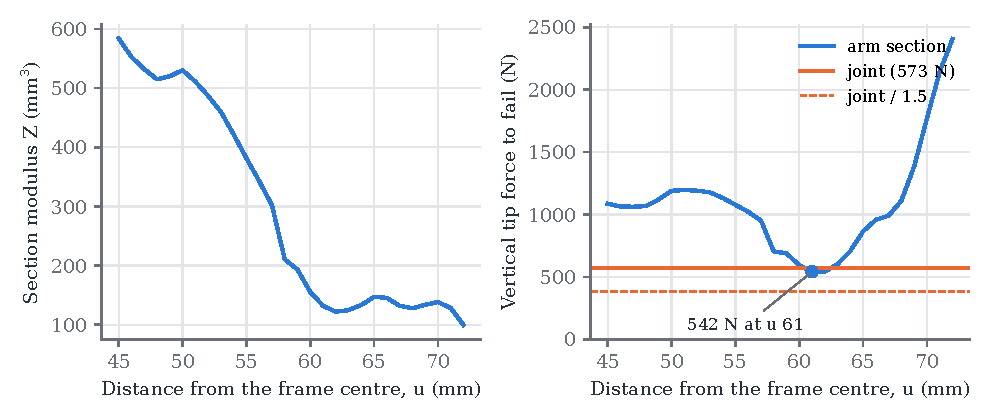
\includegraphics[width=\linewidth]{plot_capacity}
\caption{Left: section modulus of the printed arm for vertical bending along its length. Right: the vertical tip force that fails each section, against the joint capacity. The slim section near the motor pad fails at \SI{542}{N}, the joint at \SI{573}{N}.}\label{fig:cap-capacity}
\end{figure}

By this estimate (\cref{fig:cap-capacity}) the arm is marginally the weaker element, but 0.95 lies inside the scatter of both estimates: the joint's bearing allowable is assumed equal to $S_{xy}$, and the arm is taken to fail at first-fibre stress. Which one fails in a vertical overload is not controlled. A margin of 1.5 needs a ratio of 0.67 or less. The vertical failure order (R4) is not met.

Sideways the order holds with a factor of 8.5, because the fork resists in-plane bending with its full width. The fin root on the tub keeps a section modulus of \SI{957.2}{mm^3} where it leaves the body corner and at least \SI{792.4}{mm^3} along its length, against the \SI{390}{mm^3} it needs, so a joint failure would be in bearing at the bolt holes, not across the fin root.

\subsection{Why, from first principles}

Two facts combine. First, the frequency optimisation puts arm depth where the bending moment of the arm modes is largest, at the root and the joint, and removes material near the tip, where it moves without bending (\cref{sec:to-frequency}). The section that comes out weakest under a tip force is therefore the one near the motor, and the optimiser has no reason to make it stronger: a stiffness or frequency requirement says nothing about the order in which parts fail. Second, the joint was sized as balanced: the fin and the two prongs carry the same bearing force when $t_\text{fin} = 2t_\text{prong}$, so inside the joint neither the tub nor the arm is the weaker element. Capacity design has to be imposed on the joint and on the arm explicitly; it does not emerge from an optimisation for stiffness.

\subsection{Redesign}

The redesign makes the arm part, which is replaceable, the fuse. Either option needs a new thresholded frequency check, because the frequency margin of the print geometry is 3.4\,\% ($431.0/417 = 1.034$).
\begin{enumerate}
\item[(A)] \textbf{Prongs as the fuse.} Unbalance the joint so the prongs, which belong to the arm, are 1.5 times weaker in bearing than the fin, which belongs to the tub. With the fin at \SI{10}{mm}, prongs of \SI{3.3}{mm} give
\begin{equation}
\frac{F_{b,\text{fin}}}{F_{b,\text{prongs}}} = \frac{54.4 \times 3 \times 10}{2 \times 54.4 \times 3 \times 3.3} = \frac{1632}{1077} = 1.52.
\end{equation}
In a vertical overload the bolts then tear out of the prongs, and the tub is untouched.
\item[(B)] \textbf{A defined fuse section near the motor.} Keep the joint and limit the slim section so the ratio reaches 0.67:
\begin{equation}
Z \leq 0.67 \times \frac{M_j}{S_{xy}\,(u_m - u_j)}\,(u_m - u) = 0.67 \times \frac{21216}{54.4 \times 37.00} \times 13.25 \approx \SI{90}{mm^3},
\end{equation}
against \SI{131.9}{mm^3} now. The arm then breaks next to the motor pad.
\end{enumerate}
Option A changes only the fixed geometry of the joint, which the optimiser does not touch, so it keeps the optimised arm. Option B thins the section where the arm's bending stiffness matters least for the umbrella mode, but it lowers the strength margin of every load case at that section.
